% !TeX root = ../main.tex

\begin{frame}
  \frametitle{Setting}

  \begin{textblock*}{11cm}(1cm,2cm)
    Unknown $c$-Lipschitz function $f : D\to \R$.\vspace{1ex}

    \only<2>{Sublevel set $B_\omega$ that \emph{surrounds} $D$.}
  \end{textblock*}

  \begin{textblock*}{12cm}(0.5cm,5.5cm)
    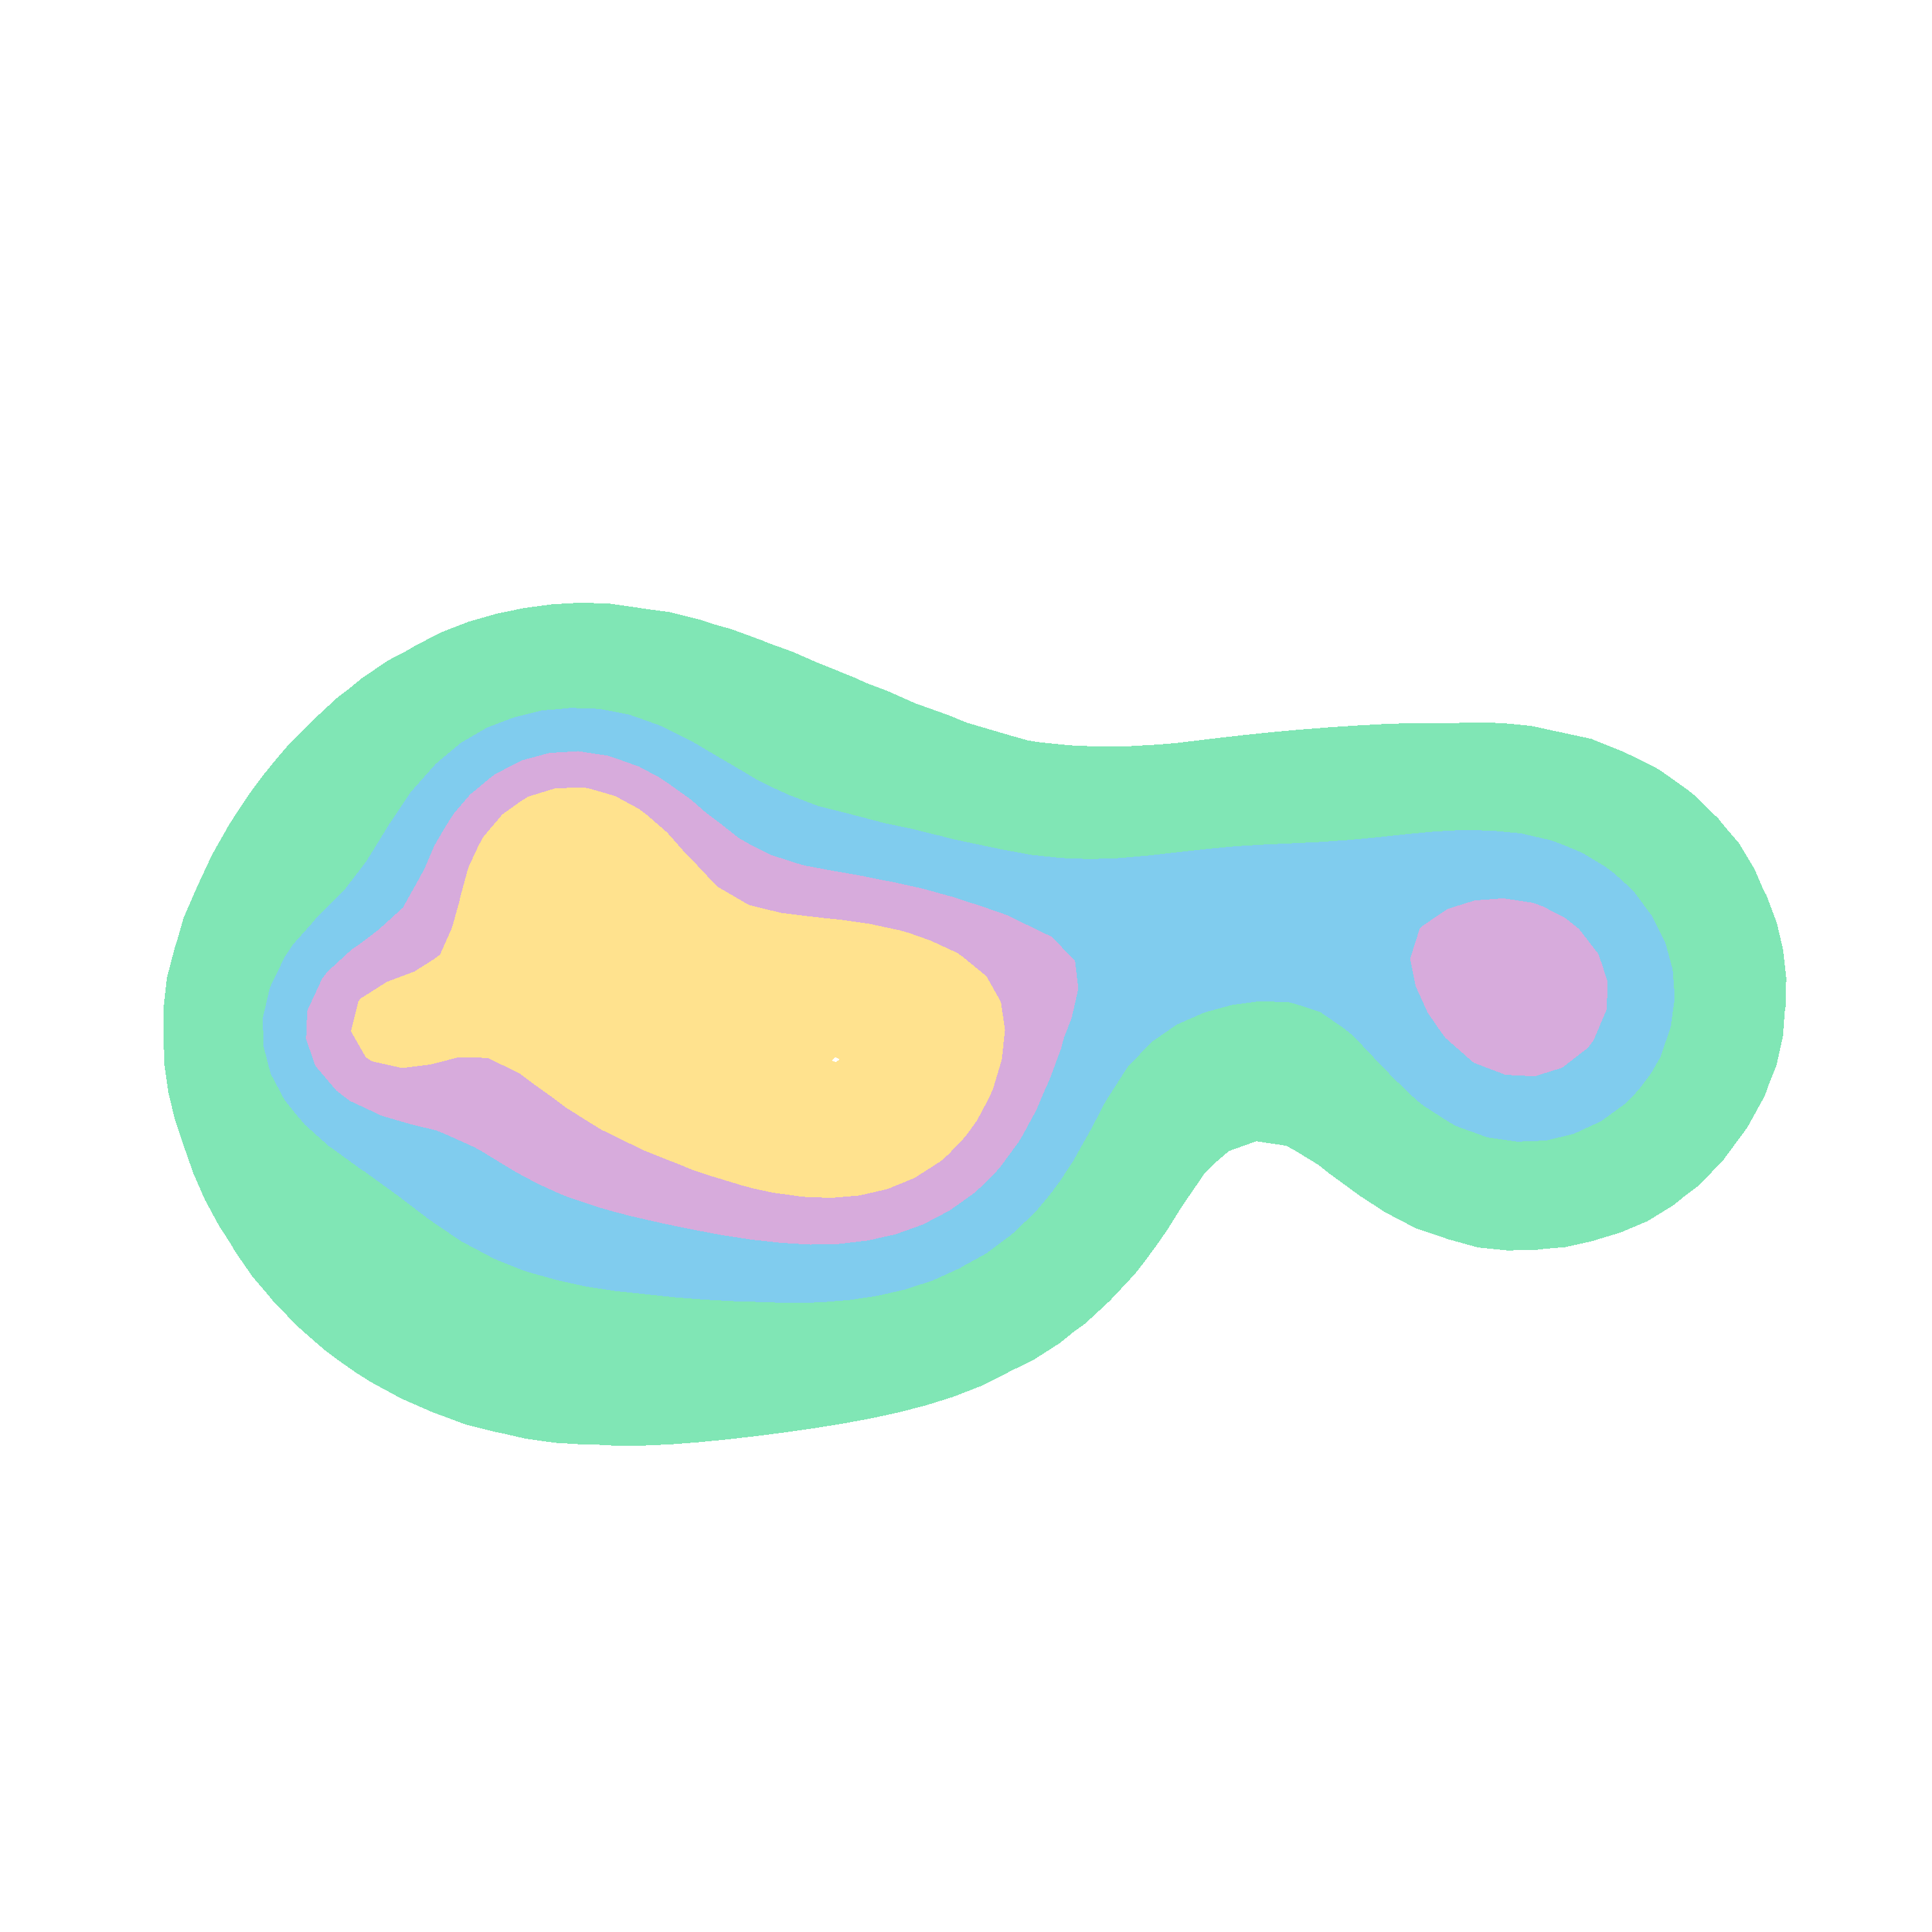
\includegraphics[trim=100 500 100 700, clip, width=0.4\textwidth]{figures/rips_dense2_2/surf}\hspace{6ex}%
    \includegraphics<2>[trim=100 500 100 700, clip, width=0.4\textwidth]{figures/rips_dense2_2/Bonly}
  \end{textblock*}

\end{frame}

\begin{frame}
  \frametitle{Input}

  \begin{textblock*}{11cm}(1cm,2cm)
    Finite sample $P\subset D$ of $f$ and $\delta > 0$.\vspace{1ex}

    Sub-sample $Q\subset P$.
  \end{textblock*}

  \begin{textblock*}{12cm}(0.5cm,5.5cm)
    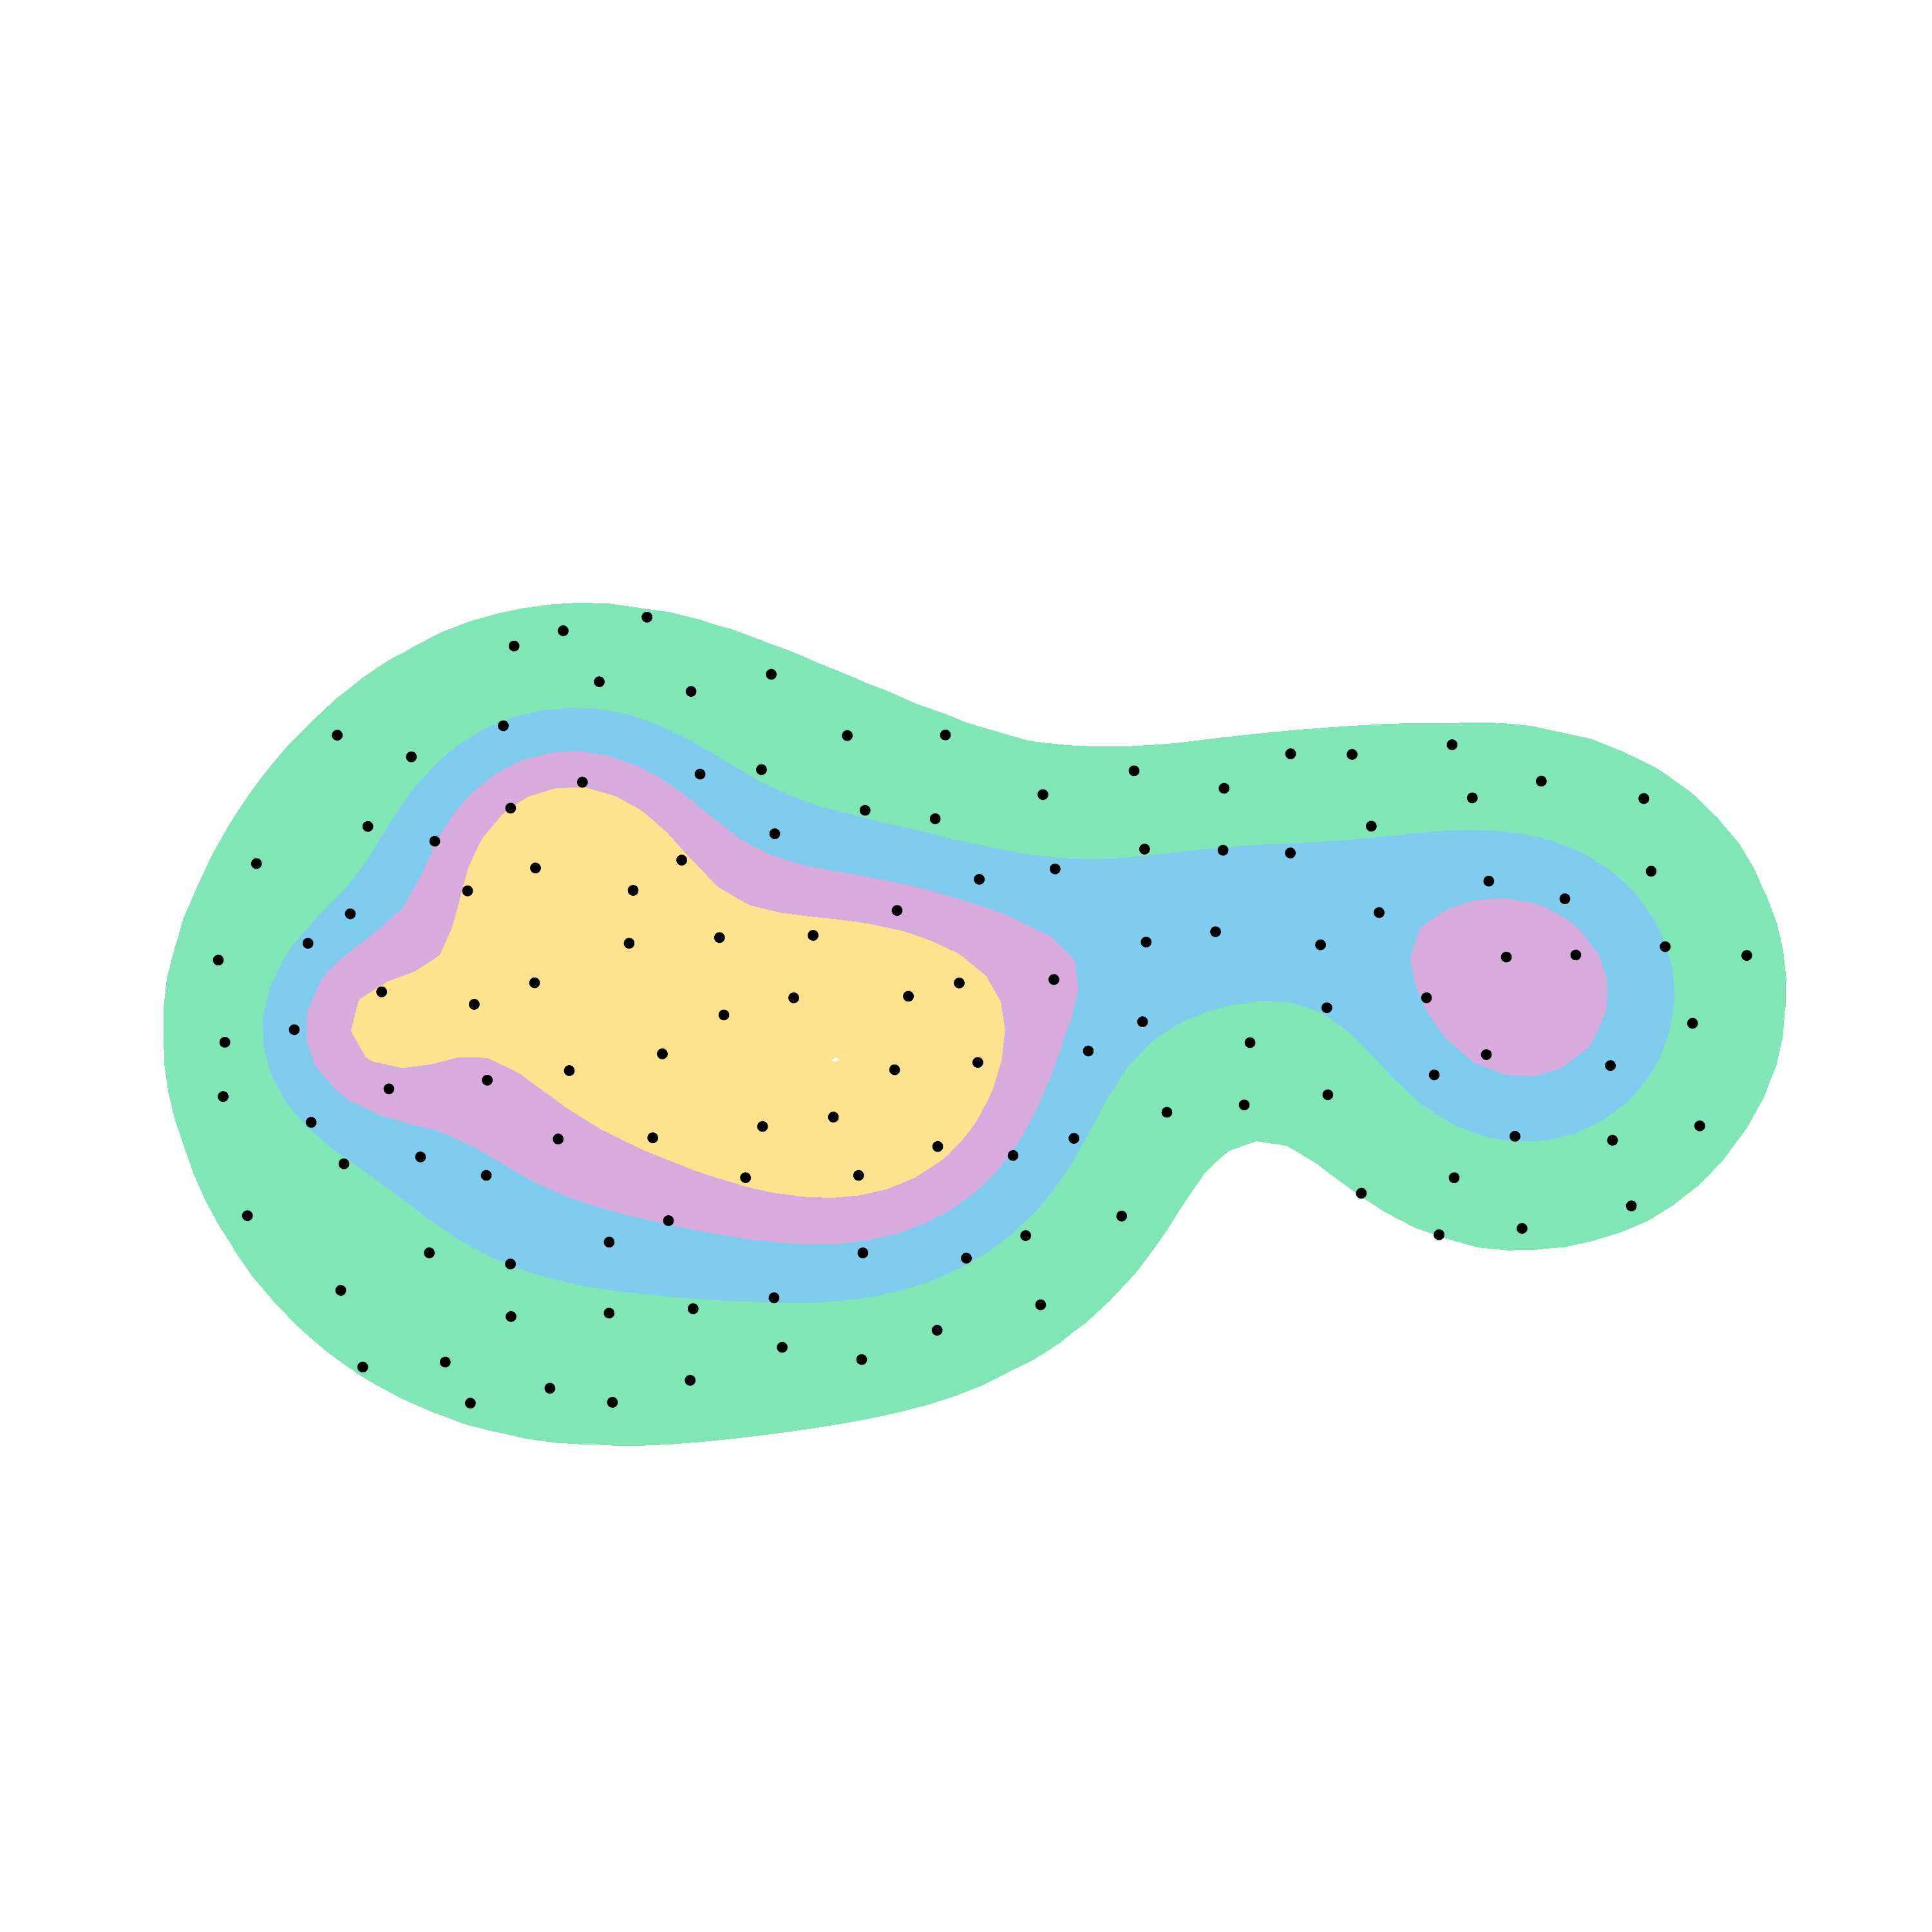
\includegraphics[trim=100 500 100 700, clip, width=0.4\textwidth]{figures/rips_dense2_2/samples}\hspace{6ex}%
    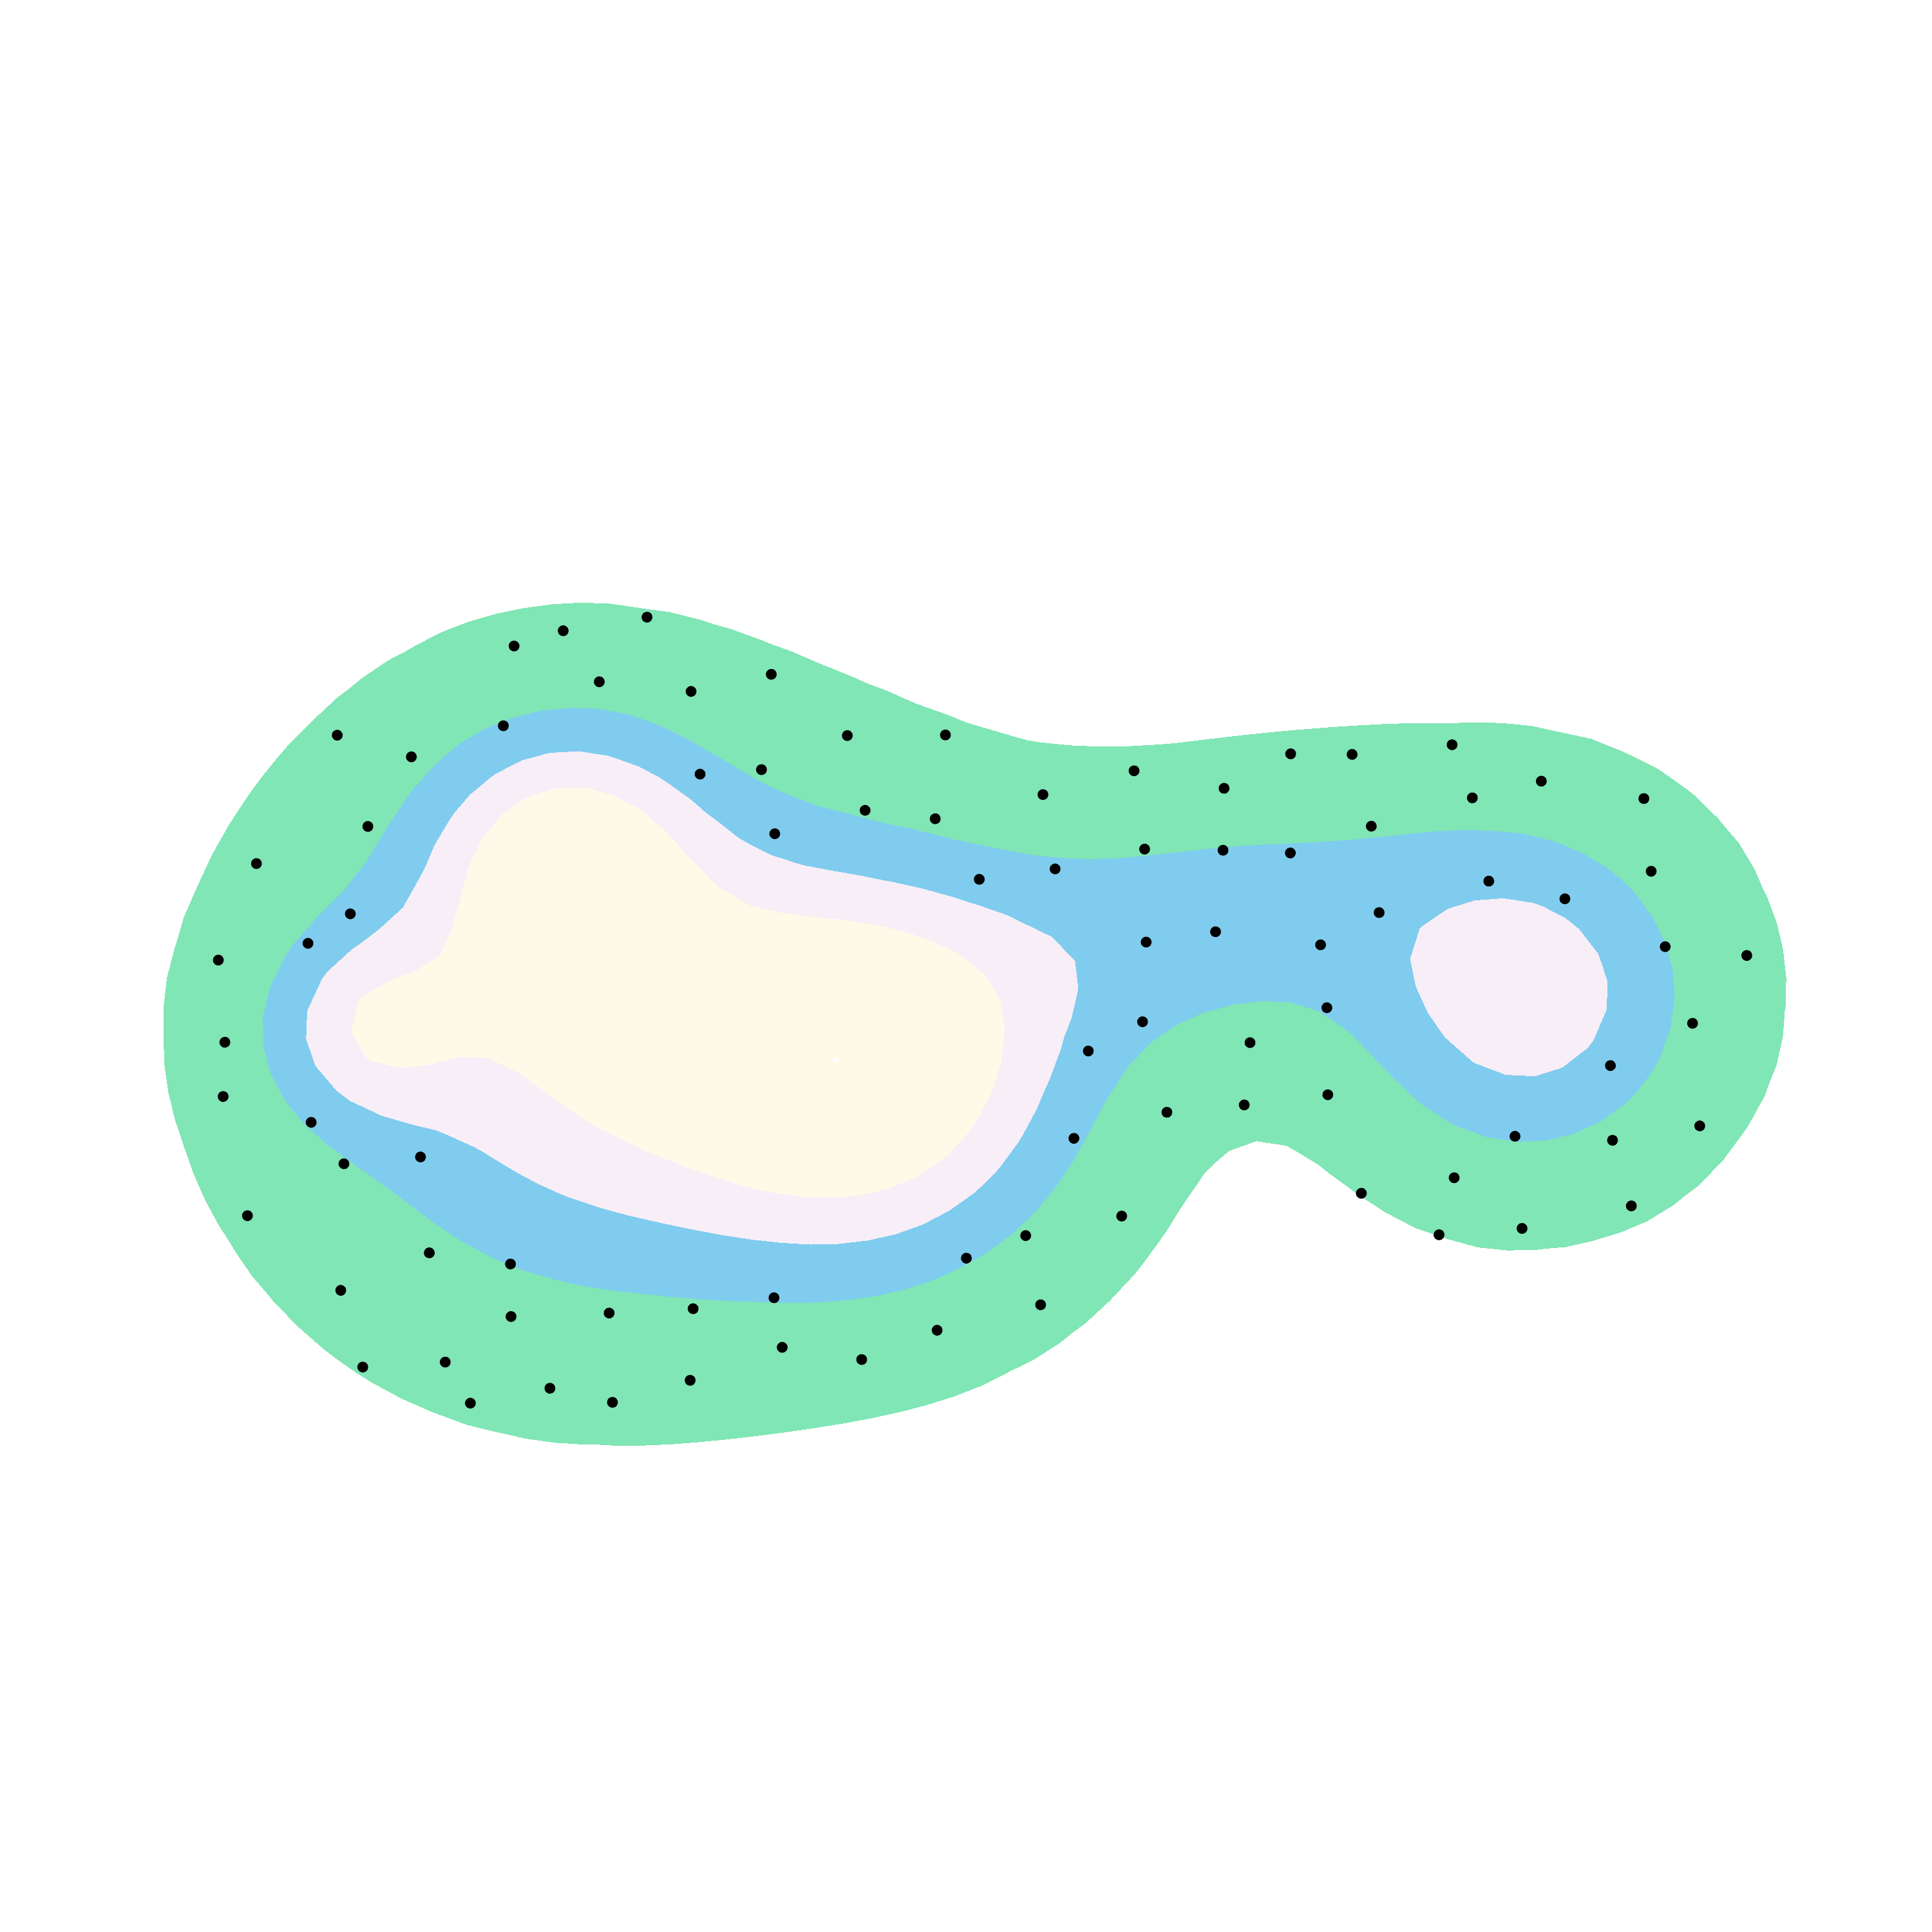
\includegraphics[trim=100 500 100 700, clip, width=0.4\textwidth]{figures/rips_dense2_2/Qsample}
  \end{textblock*}
\end{frame}

\begin{frame}
  \begin{textblock*}{12cm}(0cm,1cm)
    \begin{small}
    \begin{description}
      \item[Goal:] Confirm that $D\setminus B_\omega\subseteq P^\delta$ and $Q^\delta$ surrounds $P^\delta$ in $D$.
      \item[Method:] Check \[{\only<4-8>{\color{red}}\mathbf{dim}~\hom_d(P^\delta, Q^\delta)\geq \mathbf{dim}~\hom_d(D, B_\omega).}\]
    \end{description}
    \end{small}
  \end{textblock*}

  \begin{textblock*}{11cm}(1cm,4cm)
    \only<5-8>{{\color{red} Duality:} $\hom_d(X, Y)\cong\hom_0(\overline{Y}, \overline{X}).$}
  \end{textblock*}

  \begin{textblock*}{12cm}(0.5cm,5.5cm)
    % \includegraphics<1>[trim=100 500 100 700, clip, width=0.4\textwidth]{figures/DBA}
    \includegraphics<1-5>[trim=100 500 100 700, clip, width=0.4\textwidth]{figures/DBB}\hspace{6ex}%
    % \includegraphics<1>[trim=100 500 100 700, clip, width=0.4\textwidth]{figures/rips_dense1_Q/PQcover_nosurf}
    \includegraphics<2>[trim=100 500 100 700, clip, width=0.4\textwidth]{figures/rips_dense2_Q/PQcover_nosurf}
    \includegraphics<3-5>[trim=50 200 50 300, clip, width=0.4\textwidth]{figures/comp/PQ}%
  \end{textblock*}

  \begin{textblock*}{11cm}(1cm,6cm)
    \centering
    \includegraphics<6>[width=0.8\textwidth]{figures/balloons1}%
    \includegraphics<7>[width=0.8\textwidth]{figures/balloons2}%
    \includegraphics<8>[width=0.8\textwidth]{figures/balloons3}
  \end{textblock*}
\end{frame}

\begin{frame}
  \begin{textblock*}{12cm}(0cm,1cm)
    \begin{small}
    \begin{description}
      \item[Goal:] Confirm that $D\setminus B_\omega\subseteq P^\delta$ and $Q^\delta$ surrounds $P^\delta$ in $D$.
      \item[Method:] Check
      \[%
        \only<1>{{\color{red}\mathbf{dim}~\hom_d(P^\delta, Q^\delta)}} %
        % \only<2-6>{\mathbf{dim}~\hom_0(\overline{Q^\delta},\overline{P^\delta})}\geq%
        \only<2-4>{\mathbf{dim}~\hom_0(\overline{Q^\delta},\overline{P^\delta})}\geq%
        \only<1-3>{{\only<3>{\color{red}}\mathbf{dim}~\hom_d(D, B_\omega).}}%
        \only<4>{\mathbf{dim}~\hom_0(\overline{B_\omega},\overline{D}).}%
        % \only<4-5>{{\only<5>{\color{red}}\mathbf{dim}~\hom_0(\overline{B_\omega},\overline{D}).}}%
        % \only<6>{\mathbf{dim}~\hom_0(D\setminus B_\omega).}%
      \]
    \end{description}
    \end{small}
  \end{textblock*}

  \begin{textblock*}{11cm}(1cm,4cm)
    \only<1-4>{{\color{red} Duality:} $\hom_d(X, Y)\cong\hom_0(\overline{Y}, \overline{X}).$}%
    % \only<5-6>{{\color{red} Surrounding:} $\hom_0(D\setminus B_\omega))\cong\hom_0(\overline{B_\omega}, \overline{D}).$}
  \end{textblock*}

  % \begin{textblock*}{12cm}(0.75cm,5cm)
  %   \includegraphics<1-3>[trim=50 250 50 300, clip, width=0.4\textwidth]{figures/comp/surf}\hspace{6ex}%
  %   % \includegraphics<4->[trim=150 250 50 300, clip, width=0.4\textwidth]{figures/comp/DBcomp}\hspace{6ex}%\hspace{6ex}%
  %   \includegraphics<1>[trim=50 250 50 300, clip, width=0.4\textwidth]{figures/comp/PQ}%
  %   \includegraphics<2-3>[trim=50 250 50 300, clip, width=0.4\textwidth]{figures/comp/PQcomp}%
  % \end{textblock*}

  \begin{textblock*}{12cm}(0.75cm,5.5cm)
    \includegraphics<1-3>[trim=50 250 50 300, clip, width=0.4\textwidth]{figures/comp/surf}%
    \includegraphics<4>[trim=50 250 50 300, clip, width=0.4\textwidth]{figures/comp/DBcomp}\hspace{6ex}%
    % \includegraphics<4-5>[trim=50 250 50 300, clip, width=0.4\textwidth]{figures/comp/DBcomp}%
    % \includegraphics<6>[trim=50 250 50 300, clip, width=0.4\textwidth]{figures/comp/Bint}\hspace{6ex}%
    \includegraphics<1>[trim=50 250 50 300, clip, width=0.4\textwidth]{figures/comp/PQ}%
    \includegraphics<2-3>[trim=50 250 50 300, clip, width=0.4\textwidth]{figures/comp/PQcomp}%
    \includegraphics<4>[trim=50 250 50 300, clip, width=0.4\textwidth]{figures/comp/PQcomp}
    % \includegraphics<4-6>[trim=50 250 50 300, clip, width=0.4\textwidth]{figures/comp/PQcomp}
  \end{textblock*}
\end{frame}

\begin{frame}
  \begin{textblock*}{12cm}(0cm,1cm)
    \begin{small}
    \begin{description}
      \item[Goal:] {\color{red} Confirm that $D\setminus B_\omega\subseteq P^\delta$ and $Q^\delta$ surrounds $P^\delta$ in $D$.}
      \item[Method:] Check \[\mathbf{dim}~\hom_0(\overline{Q^\delta},\overline{P^\delta})\geq \mathbf{dim}~\hom_0(\overline{B}, \overline{D}).\]
    \end{description}
    \end{small}
  \end{textblock*}

  \begin{textblock*}{11cm}(1cm,4cm)
    \only<2>{Let $\ell : \hom_0(\overline{B}, \overline{D})\to \hom_0(\overline{Q^\delta}, \overline{P^\delta})$}
  \end{textblock*}

  \begin{textblock*}{12cm}(0.75cm,5.5cm)
    
\includegraphics[trim=50 250 50 300, clip, width=0.4\textwidth]{figures/comp/DBcomp}\hspace{6ex}%
    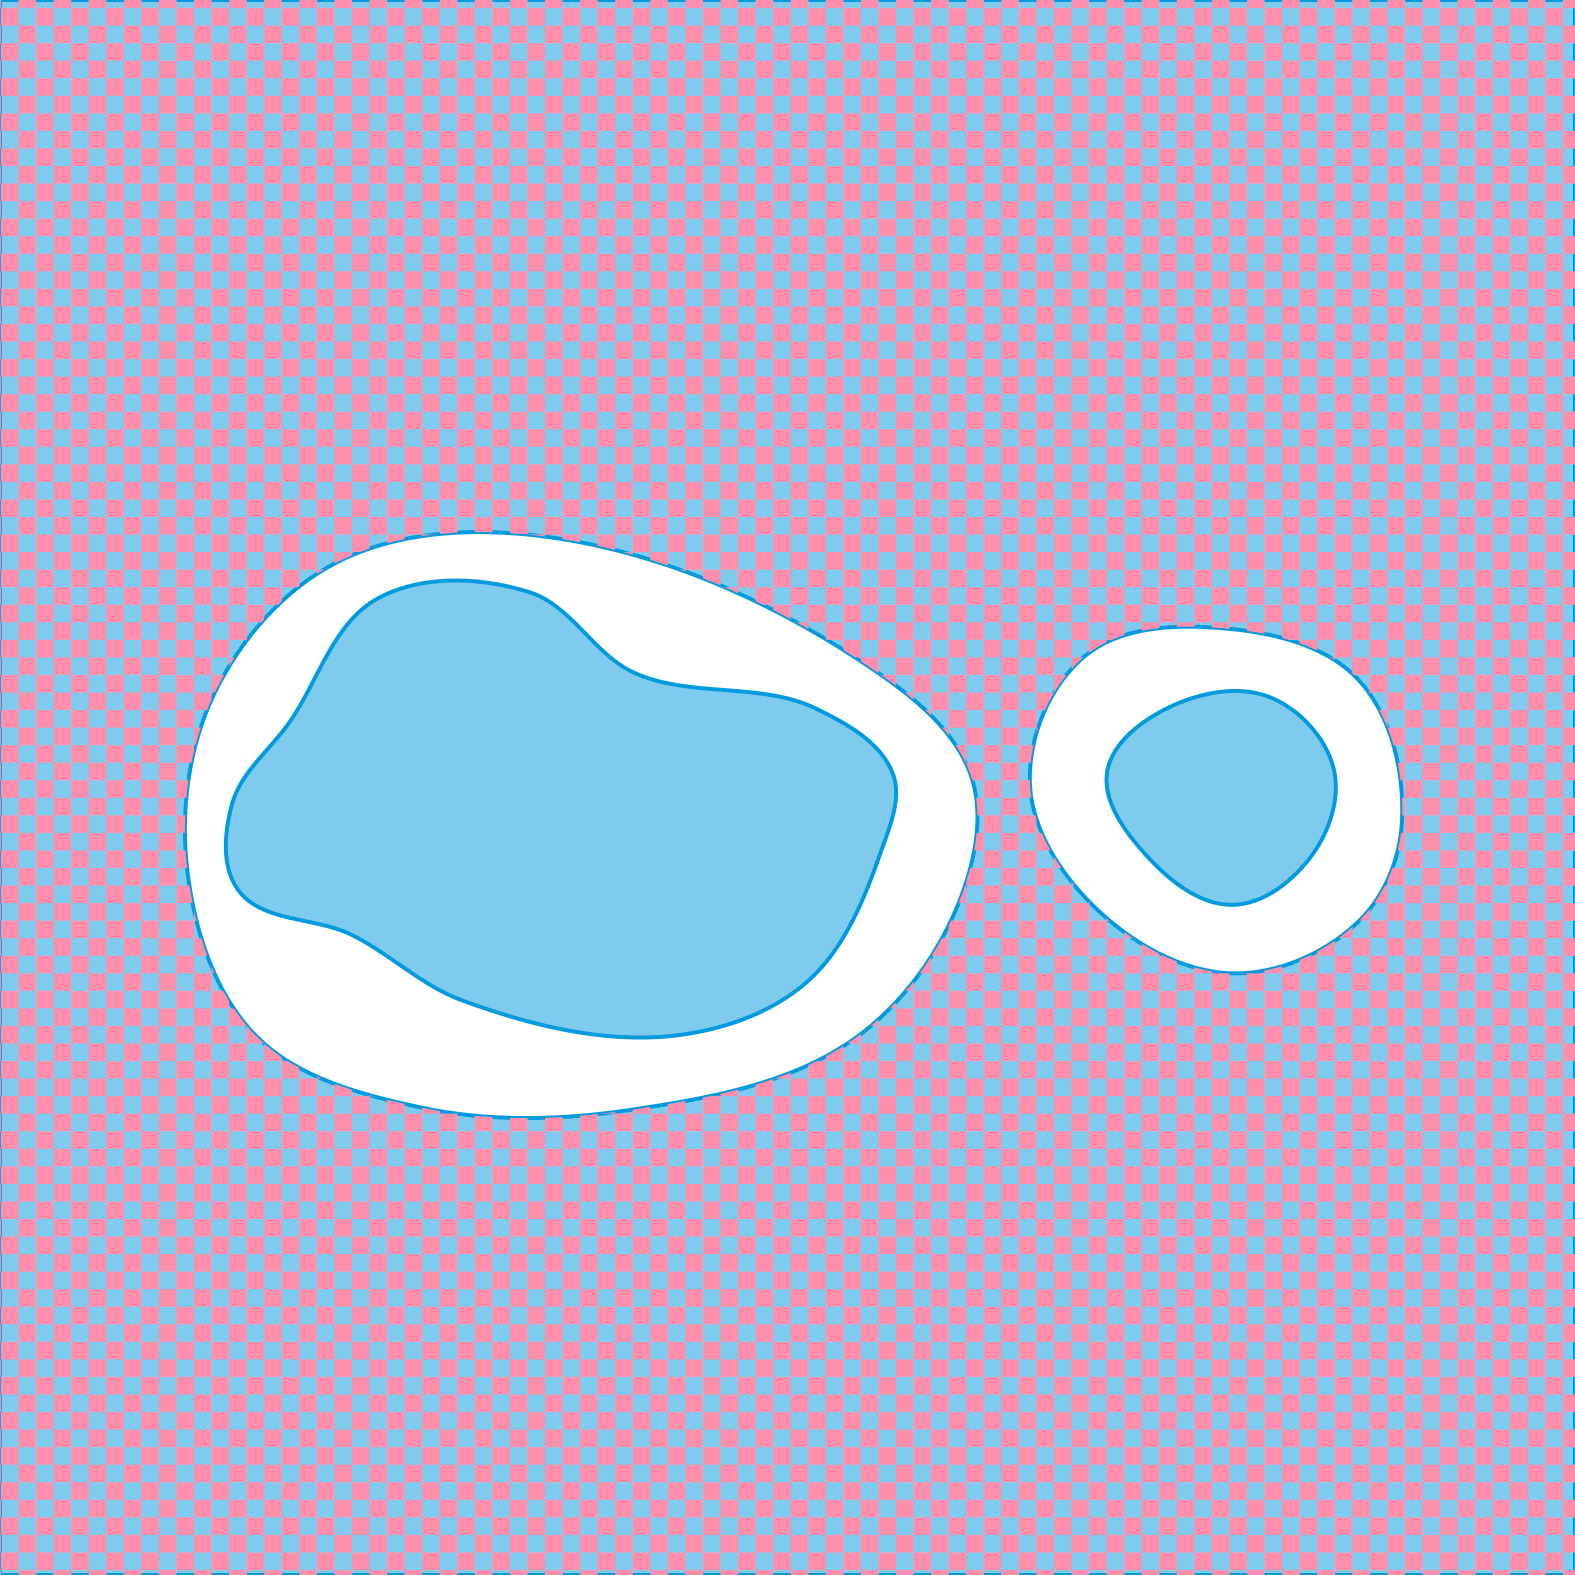
\includegraphics[trim=50 250 50 300, clip, width=0.4\textwidth]{figures/comp/PQcomp}
  \end{textblock*}
\end{frame}

% \begin{frame}
%   \frametitle{Properties of Surrounding pairs}
%
%   \begin{textblock*}{11cm}(1cm,2cm)
%     \begin{small}
%       Surrounding pair $(D, B)$.\vspace{1ex}
%
%       \only<2,3>{Pair $(P^\delta, Q^\delta)$ with $P^\delta\subseteq D$, $Q^\delta\subseteq P^\delta\cap B$.\vspace{1ex}}
%
%       \only<3>{Let $\ell : \hom_0(\overline{B}, \overline{D})\to \hom_0(\overline{Q^\delta}, \overline{P^\delta})$}
%     \end{small}
%   \end{textblock*}
%
%   \begin{textblock*}{12cm}(0.75cm,5cm)
%     \includegraphics<1,2>[trim=50 250 50 300, clip, width=0.4\textwidth]{figures/comp/surf}%
%     \includegraphics<3>[trim=50 250 50 300, clip, width=0.4\textwidth]{figures/comp/DBcomp}\hspace{6ex}%
%     \includegraphics<2>[trim=50 250 50 300, clip, width=0.4\textwidth]{figures/comp/PQ}%
%     \includegraphics<3>[trim=50 250 50 300, clip, width=0.4\textwidth]{figures/comp/PQcomp}
%   \end{textblock*}
% \end{frame}
%
\begin{frame}
  \begin{textblock*}{12cm}(0cm,1cm)
    \begin{small}
    \begin{description}
      \item[Goal:] {\color{red} Confirm that $D\setminus B_\omega\subseteq P^\delta$ and $Q^\delta$ surrounds $P^\delta$ in $D$.}
      \item[Method:] Check \[\mathbf{dim}~\hom_0(\overline{Q^\delta},\overline{P^\delta})\geq \mathbf{dim}~\hom_0(\overline{B}, \overline{D}).\]
    \end{description}
    \end{small}
  \end{textblock*}

  \begin{textblock*}{11cm}(1cm,3.3cm)
    \begin{small}
      \begin{lemma}\label{lem:coverage}
        If $\ell$ is injective then $D\setminus B_\omega\subseteq P^\delta$ and $Q^\delta$ surrounds $P^\delta$ in $D$.
      \end{lemma}
    \end{small}
  \end{textblock*}

  \begin{textblock*}{12cm}(0.75cm,5.5cm)
    \includegraphics<1>[trim=50 250 50 300, clip, width=0.4\textwidth]{figures/comp/DBcomp}\only<1>{\hspace{6ex}}%
    \includegraphics<1>[trim=50 250 50 300, clip, width=0.4\textwidth]{figures/comp/PQcomp}%
    \includegraphics<2>[trim=50 250 50 300, clip, width=0.4\textwidth]{figures/comp/surf}\only<2>{\hspace{6ex}}%
    \includegraphics<2>[trim=50 250 50 300, clip, width=0.4\textwidth]{figures/comp/PQnocov}%
    \includegraphics<3,4>[trim=50 250 50 300, clip, width=0.4\textwidth]{figures/comp/DBcomp}\only<3,4>{\hspace{6ex}}%
    \includegraphics<3>[trim=50 250 50 300, clip, width=0.4\textwidth]{figures/comp/PQnocov_comp}%
    \includegraphics<4>[trim=50 250 50 300, clip, width=0.4\textwidth]{figures/comp/PQnocov_comp-spread}%
    \includegraphics<5>[trim=50 250 50 300, clip, width=0.4\textwidth]{figures/comp/Bint}\only<5>{\hspace{6ex}}%
    \includegraphics<5>[trim=50 250 50 300, clip, width=0.4\textwidth]{figures/comp/Qno_int}
  \end{textblock*}
\end{frame}

\begin{frame}
  \begin{textblock*}{12cm}(0cm,1cm)
    \begin{small}
    \begin{description}
      \item[Goal:] {\color{red} Confirm that $D\setminus B_\omega\subseteq P^\delta$ and $Q^\delta$ surrounds $P^\delta$ in $D$.}
      \item[Method:] Check \[\mathbf{dim}~\hom_0(\overline{Q^\delta},\overline{P^\delta})\geq \mathbf{dim}~\hom_0(\overline{B}, \overline{D}).\]
    \end{description}
    \end{small}
  \end{textblock*}

  \begin{textblock*}{11cm}(1cm,3.3cm)
    \begin{small}
      \begin{lemma}\label{lem:coverage}
        If $\ell$ is injective then $D\setminus B_\omega\subseteq P^\delta$ and $Q^\delta$ surrounds $P^\delta$ in $D$.
      \end{lemma}
    \end{small}
  \end{textblock*}

  \begin{textblock*}{12cm}(0.75cm,5.5cm)
    \includegraphics<1>[trim=50 250 50 300, clip, width=0.4\textwidth]{figures/comp/surf}\only<1>{\hspace{6ex}}%
    \includegraphics<1>[trim=50 250 50 300, clip, width=0.4\textwidth]{figures/comp/PQnosur}%
    \includegraphics<2,3>[trim=50 250 50 300, clip, width=0.4\textwidth]{figures/comp/DBcomp}\only<2,3>{\hspace{6ex}}%
    \includegraphics<2>[trim=50 250 50 300, clip, width=0.4\textwidth]{figures/comp/PQnosur_comp}%
    \includegraphics<3>[trim=50 250 50 300, clip, width=0.4\textwidth]{figures/comp/PQnosur_comp-spread}%
    \includegraphics<4>[trim=50 250 50 300, clip, width=0.4\textwidth]{figures/comp/Bint}\only<4>{\hspace{6ex}}%
    \includegraphics<4>[trim=50 250 50 300, clip, width=0.4\textwidth]{figures/comp/Qno_int}%
  \end{textblock*}
\end{frame}

\begin{frame}
  \begin{textblock*}{12cm}(0cm,1cm)
    \begin{small}
    \begin{description}
      \item[Goal:] \only<1>{{\color{red} Confirm that $D\setminus B_\omega\subseteq P^\delta$ and $Q^\delta$ surrounds $P^\delta$ in $D$.}}%
                    \only<2>{Show $\ell : \hom_0(\overline{B_\omega}, \overline{D})\to \hom_0(\overline{Q^\delta},\overline{P^\delta})$ is injective}
      \item[Method:] Check \[\mathbf{dim}~\hom_0(\overline{Q^\delta},\overline{P^\delta})\geq \mathbf{dim}~\hom_0(\overline{B}, \overline{D}).\]
    \end{description}
    \end{small}
  \end{textblock*}

  \begin{textblock*}{11cm}(1cm,3.3cm)
    \begin{small}
      \begin{lemma}\label{lem:coverage}
        If $\ell$ is injective then $D\setminus B_\omega\subseteq P^\delta$ and $Q^\delta$ surrounds $P^\delta$ in $D$.
      \end{lemma}
    \end{small}
  \end{textblock*}

  \begin{textblock*}{12cm}(0.75cm,5.5cm)
    \includegraphics<1-2>[trim=50 250 50 300, clip, width=0.4\textwidth]{figures/comp/DBcomp}\hspace{6ex}%
    \includegraphics<1-2>[trim=50 250 50 300, clip, width=0.4\textwidth]{figures/comp/PQcomp}%
  \end{textblock*}
\end{frame}

\begin{frame}
  \begin{textblock*}{12cm}(0cm,1cm)
    \begin{small}
    \begin{description}
      \item[Goal:] Show $\ell : \hom_0(\overline{B_\omega}, \overline{D})\to \hom_0(\overline{Q^\delta},\overline{P^\delta})$ is injective
      \item[Method:] Check \[%
        \mathbf{dim}~\hom_0(\overline{Q^\delta},\overline{P^\delta})\geq%
        \only<1-2>{{\only<2>{\color{red}}\mathbf{dim}~\hom_0(\overline{B}, \overline{D}).}}%
        \only<3>{\mathbf{dim}~\hom_0(D\setminus B_\omega).}\]
    \end{description}
    \end{small}
  \end{textblock*}

  \begin{textblock*}{11cm}(1cm,4cm)
    {\color{red} Surrounding:} $\hom_0(D\setminus B_\omega))\cong\hom_0(\overline{B_\omega}, \overline{D}).$
  \end{textblock*}

  % \begin{textblock*}{12cm}(0.75cm,5cm)
  %   \includegraphics<1-3>[trim=50 250 50 300, clip, width=0.4\textwidth]{figures/comp/surf}\hspace{6ex}%
  %   % \includegraphics<4->[trim=150 250 50 300, clip, width=0.4\textwidth]{figures/comp/DBcomp}\hspace{6ex}%\hspace{6ex}%
  %   \includegraphics<1>[trim=50 250 50 300, clip, width=0.4\textwidth]{figures/comp/PQ}%
  %   \includegraphics<2-3>[trim=50 250 50 300, clip, width=0.4\textwidth]{figures/comp/PQcomp}%
  % \end{textblock*}

  \begin{textblock*}{12cm}(0.75cm,5.5cm)
    \includegraphics<1-2>[trim=50 250 50 300, clip, width=0.4\textwidth]{figures/comp/DBcomp}%
    \includegraphics<3>[trim=50 250 50 300, clip, width=0.4\textwidth]{figures/comp/Bint}\hspace{6ex}%
    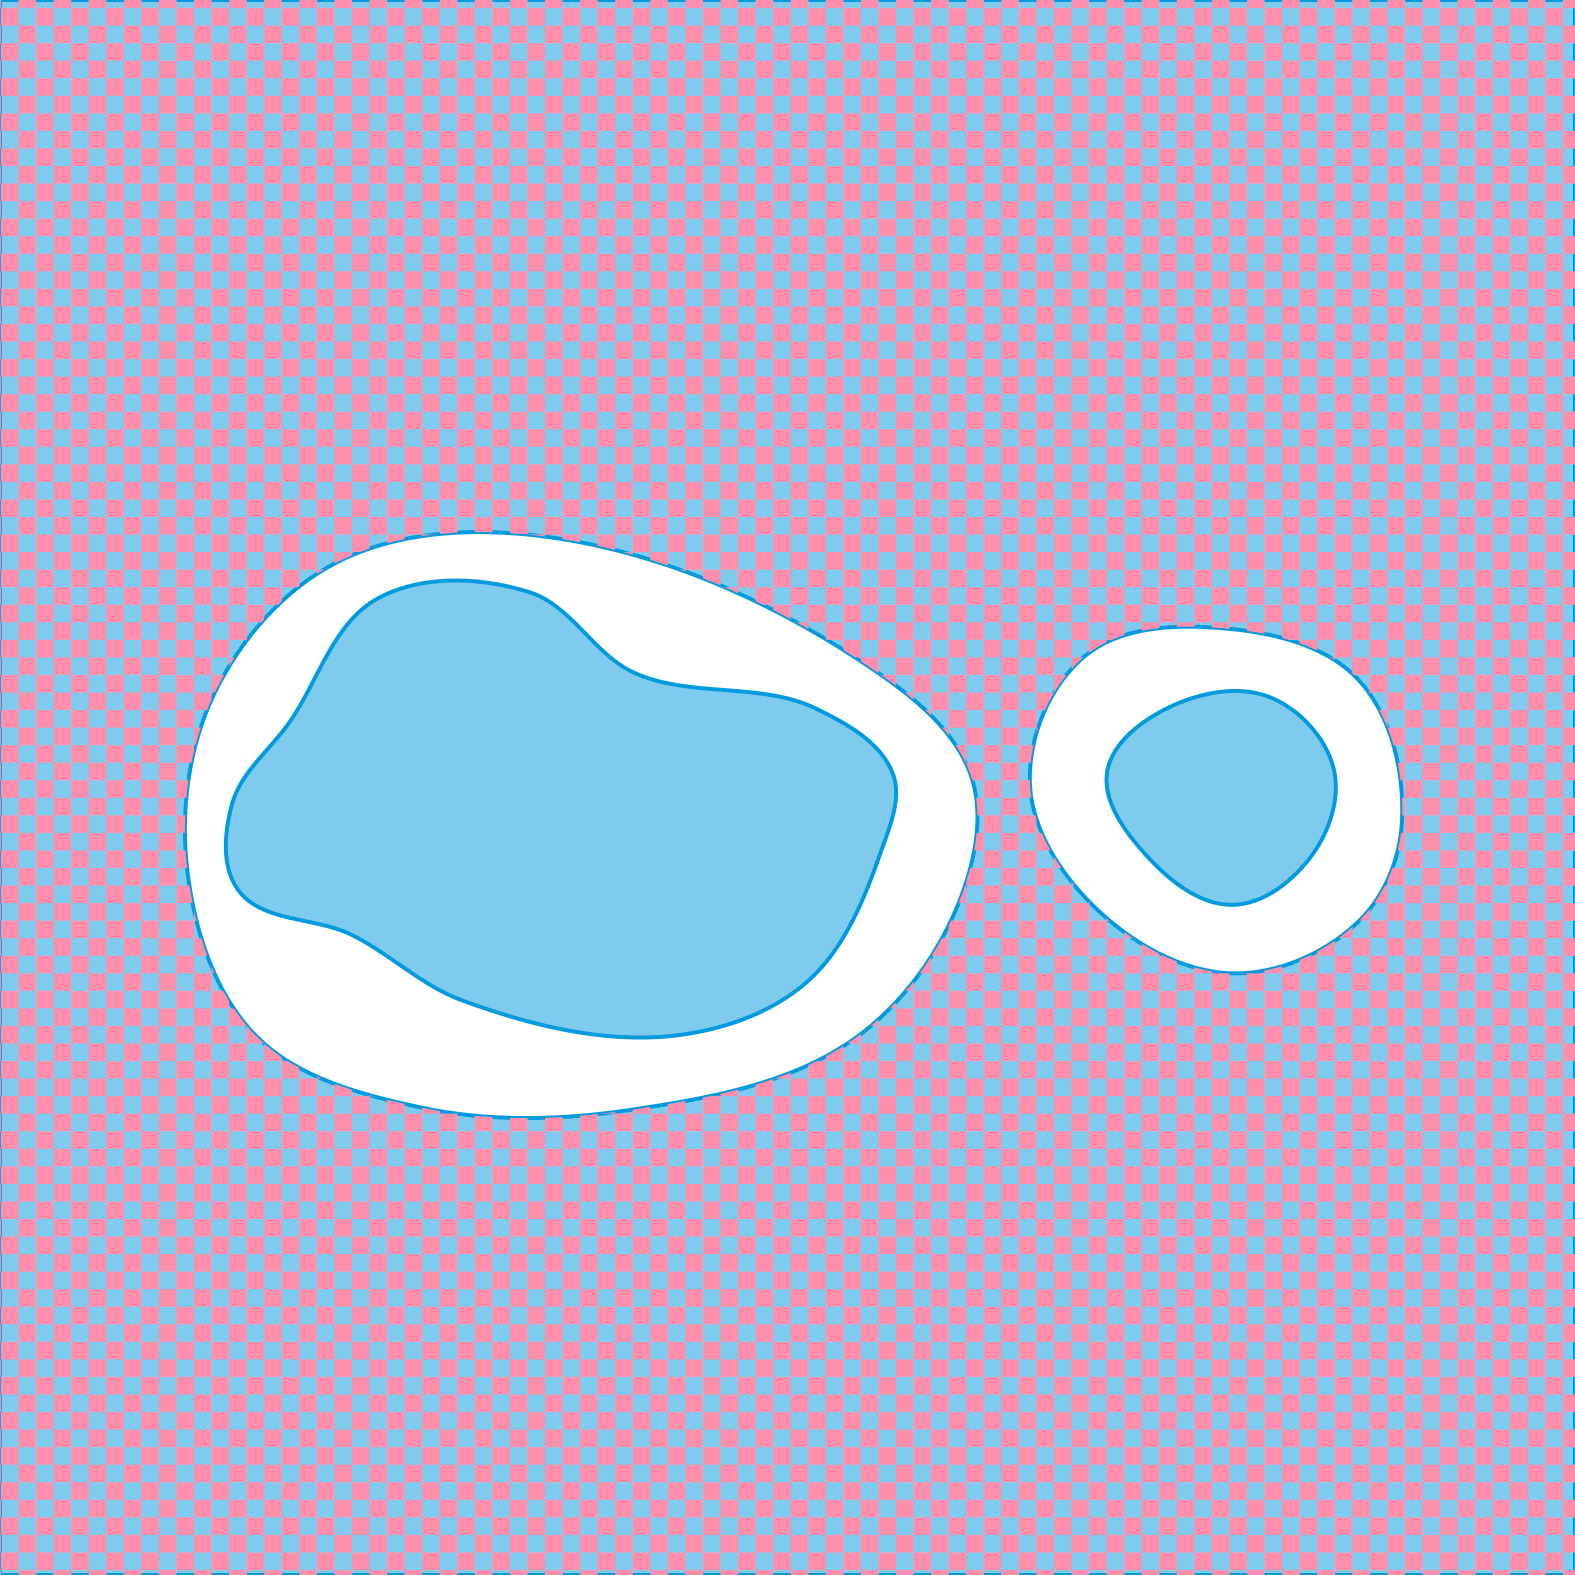
\includegraphics[trim=50 250 50 300, clip, width=0.4\textwidth]{figures/comp/PQcomp}
  \end{textblock*}
\end{frame}

\begin{frame}
  \begin{textblock*}{12cm}(0cm,1cm)
    \begin{small}
    \begin{description}
      \item[Goal:] Show $\ell : \hom_0(\overline{B_\omega}, \overline{D})\to \hom_0(\overline{Q^\delta},\overline{P^\delta})$ is injective
      \item[Method:] Check \[\mathbf{dim}~\hom_0(\overline{Q^\delta},\overline{P^\delta})\geq \mathbf{dim}~\hom_0(D\setminus B_\omega).\]
      \item[Problems:]
    \end{description}
    \end{small}
  \end{textblock*}

  \begin{textblock*}{11cm}(1cm,4.75cm)
    \begin{small}
    \begin{enumerate}[a]
      \item $\mathbf{dim}~\hom_0(\overline{Q^\delta}, \overline{P^\delta})\geq \mathbf{dim}~\hom_0(D\setminus B_\omega)\nRightarrow \ell$ injective,
      \item Cannot compute homology of offsets,
      \item $\mathbf{dim}~\hom_0(D\setminus B_\omega)$ unknown.
    \end{enumerate}
    \end{small}
  \end{textblock*}
\end{frame}
